\section{FESDModelv1 Results}
\label{sec:FESDModelv1_results}

After training all four models using FESDModelv1, the results are evaluated. Table \ref{tab:res_v1} shows the results of the testing after 50 epochs of training. The results seem promising with an accuracy in the range of 80 to 90 percent. Additionally, the Cohen's Kappa coefficient shows results in a good range.

\begin{table}[!htbp]
  \caption[Test Results of FESDModelv1]{The test results of FESDModelv1 after 50 epochs of training.}
  \label{tab:res_v1}
  \begin{tabular}{lrrrrr}
    \hline
    {} &  Percentage of positive guesses &  Accuracy &  F1-Score &  F2-Score &  Cohen's Kappa Coefficient \\
    Problem Set   &                                 &           &           &           &                            \\
    \hline
    Full Body  &                          50.417 &     0.688 &     0.458 &     0.673 &                      0.397 \\
    Half Body  &                          55.833 &     0.767 &     0.446 &     0.789 &                      0.554 \\
    Body Parts &                          79.028 &     0.779 &     0.722 &     0.842 &                      0.257 \\
    Joints     &                          70.000 &     0.892 &     0.638 &     0.918 &                      0.773 \\
    \hline
  \end{tabular}
\end{table}

To get a further understanding of these results the cofusion matrix and ROC curve were calculated. The confusion matrices can be seen in figure \ref{fig:conf_v1} and ROC curves can be seen in figure \ref{fig:roc_v1}.

\begin{figure}[!htbp]
  \centering
  \begin{subfigure}[b]{0.4\linewidth}
      \centering
      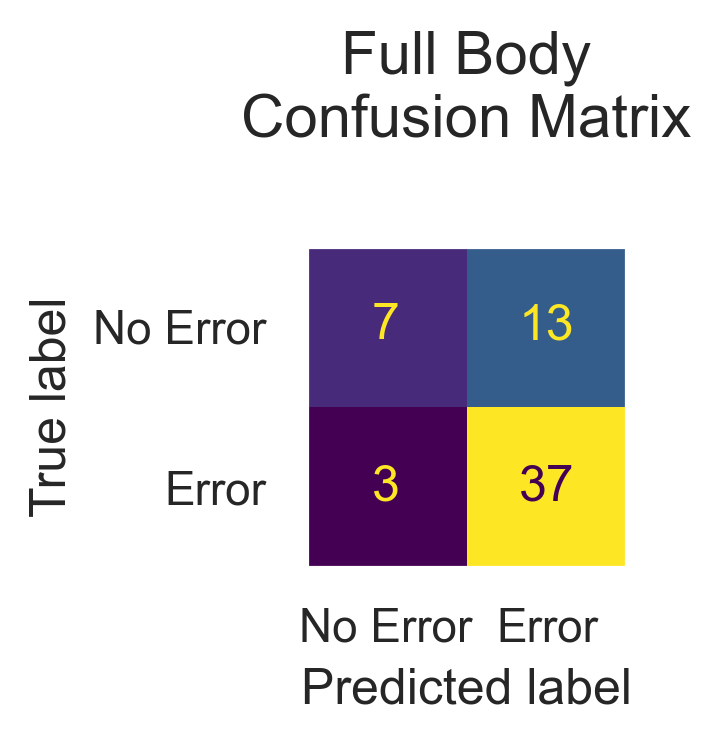
\includegraphics[width=\textwidth]{figures/Results/v1/confusion/full_together.png}
      \caption[]{Full Body Problem Set}
      \label{fig:fb_conf_v1}
  \end{subfigure}
  \hfill
  \begin{subfigure}[b]{0.4\linewidth}
      \centering
      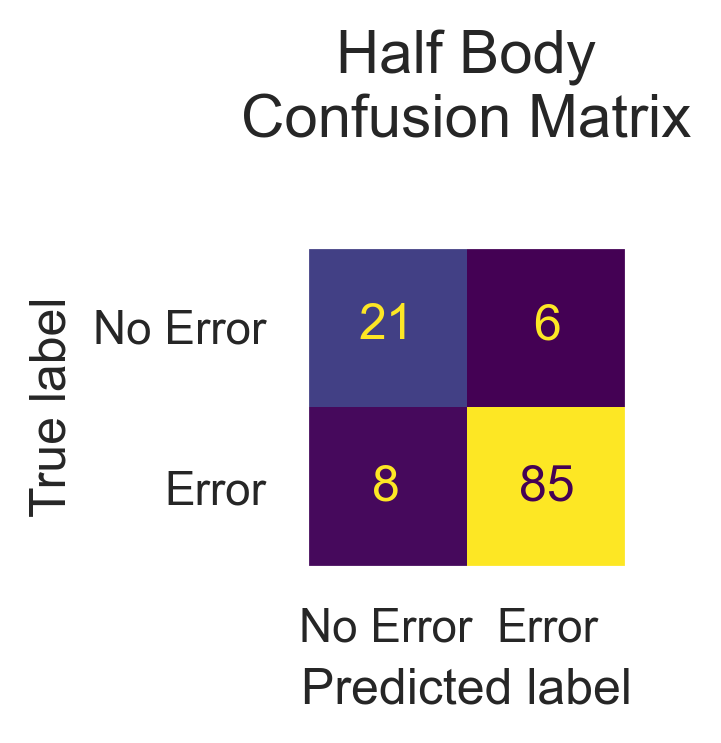
\includegraphics[width=\textwidth]{figures/Results/v1/confusion/half_together.png}
      \caption[]{Half Body Problem Set}
      \label{fig:hb_conf_v1}
  \end{subfigure}
  \hfill
  \begin{subfigure}[b]{0.4\linewidth}
      \centering
      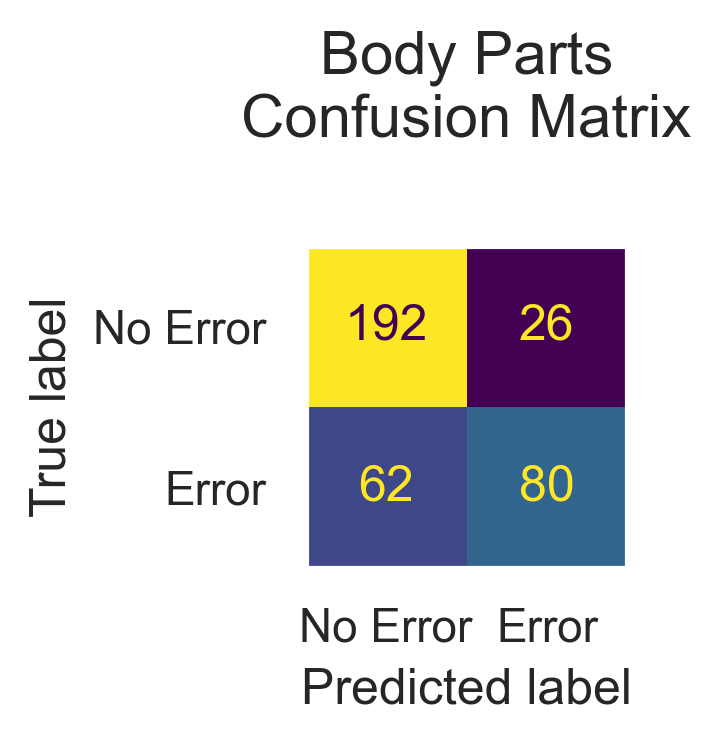
\includegraphics[width=\textwidth]{figures/Results/v1/confusion/body_parts_together.png}
      \caption[]{Body Part Problem Set}
      \label{fig:bp_conf_v1}
  \end{subfigure}
  \hfill
  \begin{subfigure}[b]{0.4\linewidth}
      \centering
      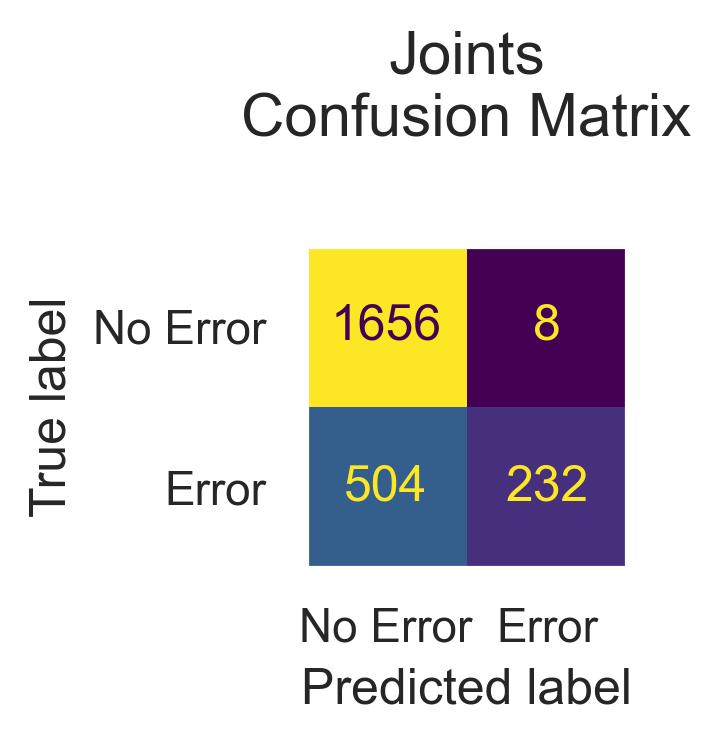
\includegraphics[width=\textwidth]{figures/Results/v1/confusion/joints_together.png}
      \caption[]{Joint Problem Set}
      \label{fig:jt_conf_v1}
  \end{subfigure}
  \caption[Confusion Matrices of FESDModelv1]{The confusion Matrices of FESDModelv1.}
  \label{fig:conf_v1}
\end{figure}


The odd looking figure \ref{fig:jt_roc_v1} can be explained using the results of the prediction. The model predicting the joint problem set is overconfident and therefore, there is only a limited number of thresholds that can be shown in the ROC curve. Therefore, the majority of the datapoints is in the upper right corner.

\begin{figure}[htbp]
  \centering
  \begin{subfigure}[b]{0.4\linewidth}
      \centering
      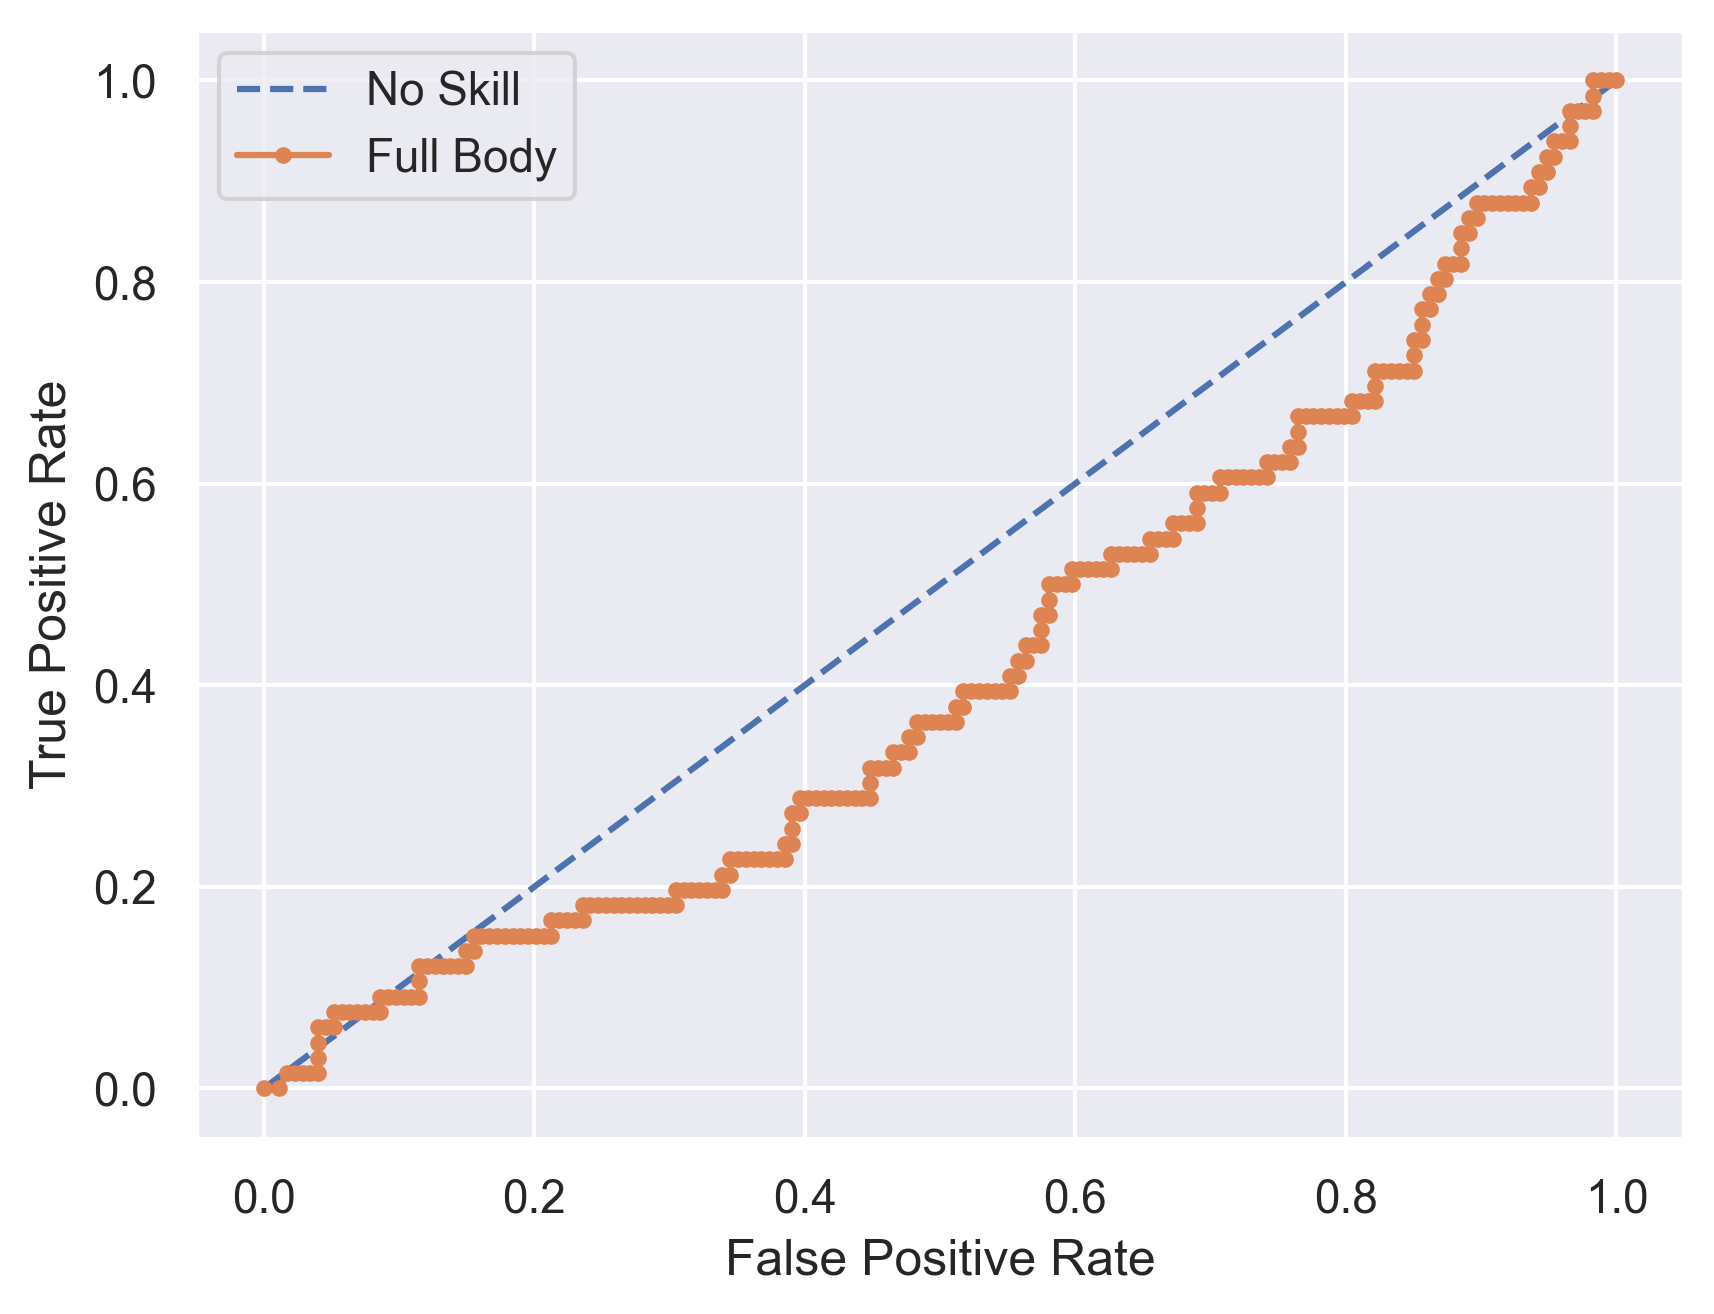
\includegraphics[width=\textwidth]{figures/Results/v1/roc/fb.png}
      \caption[]{Full Body Problem Set}
      \label{fig:fb_roc_v1}
  \end{subfigure}
  \hfill
  \begin{subfigure}[b]{0.4\linewidth}
      \centering
      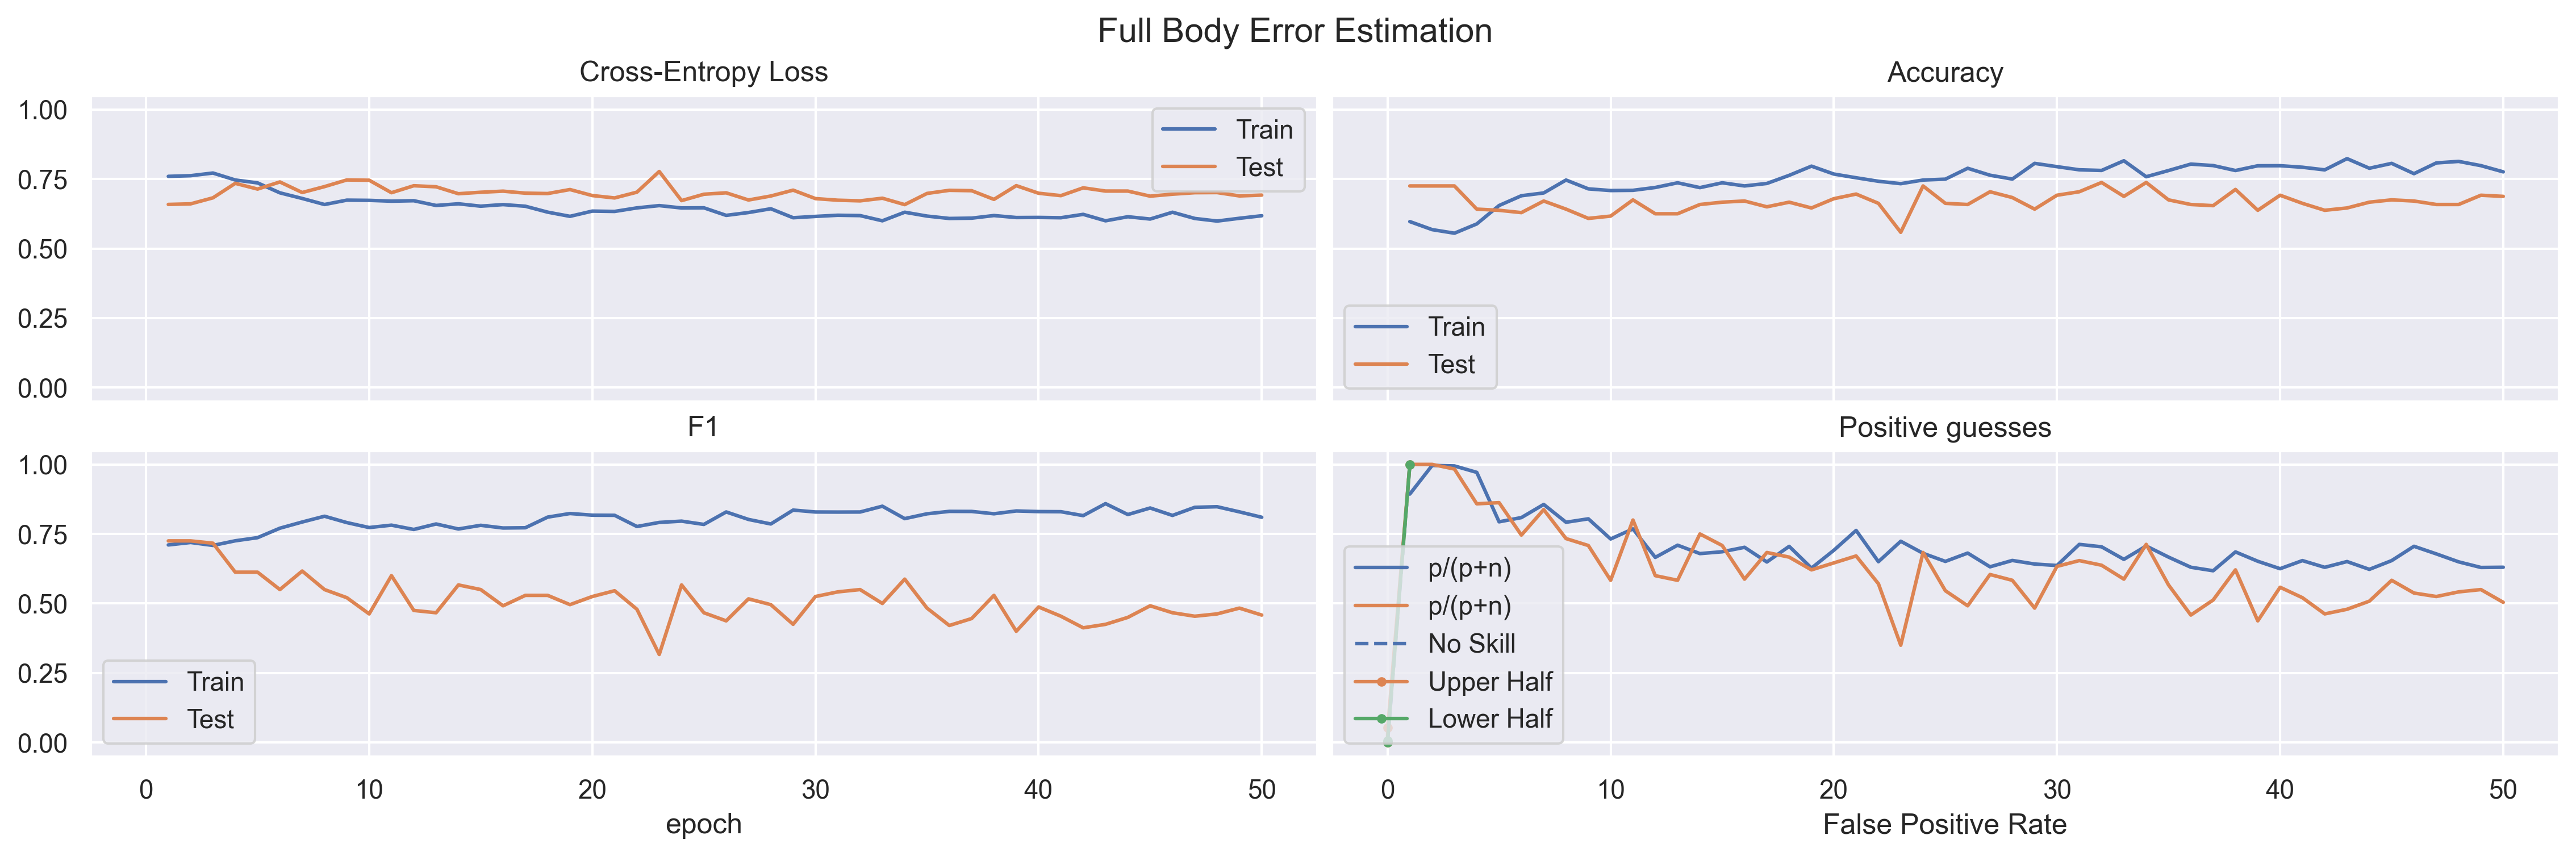
\includegraphics[width=\textwidth]{figures/Results/v1/roc/hb.png}
      \caption[]{Half Body Problem Set}
      \label{fig:hb_roc_v1}
  \end{subfigure}
  \hfill
  \begin{subfigure}[b]{0.4\linewidth}
      \centering
      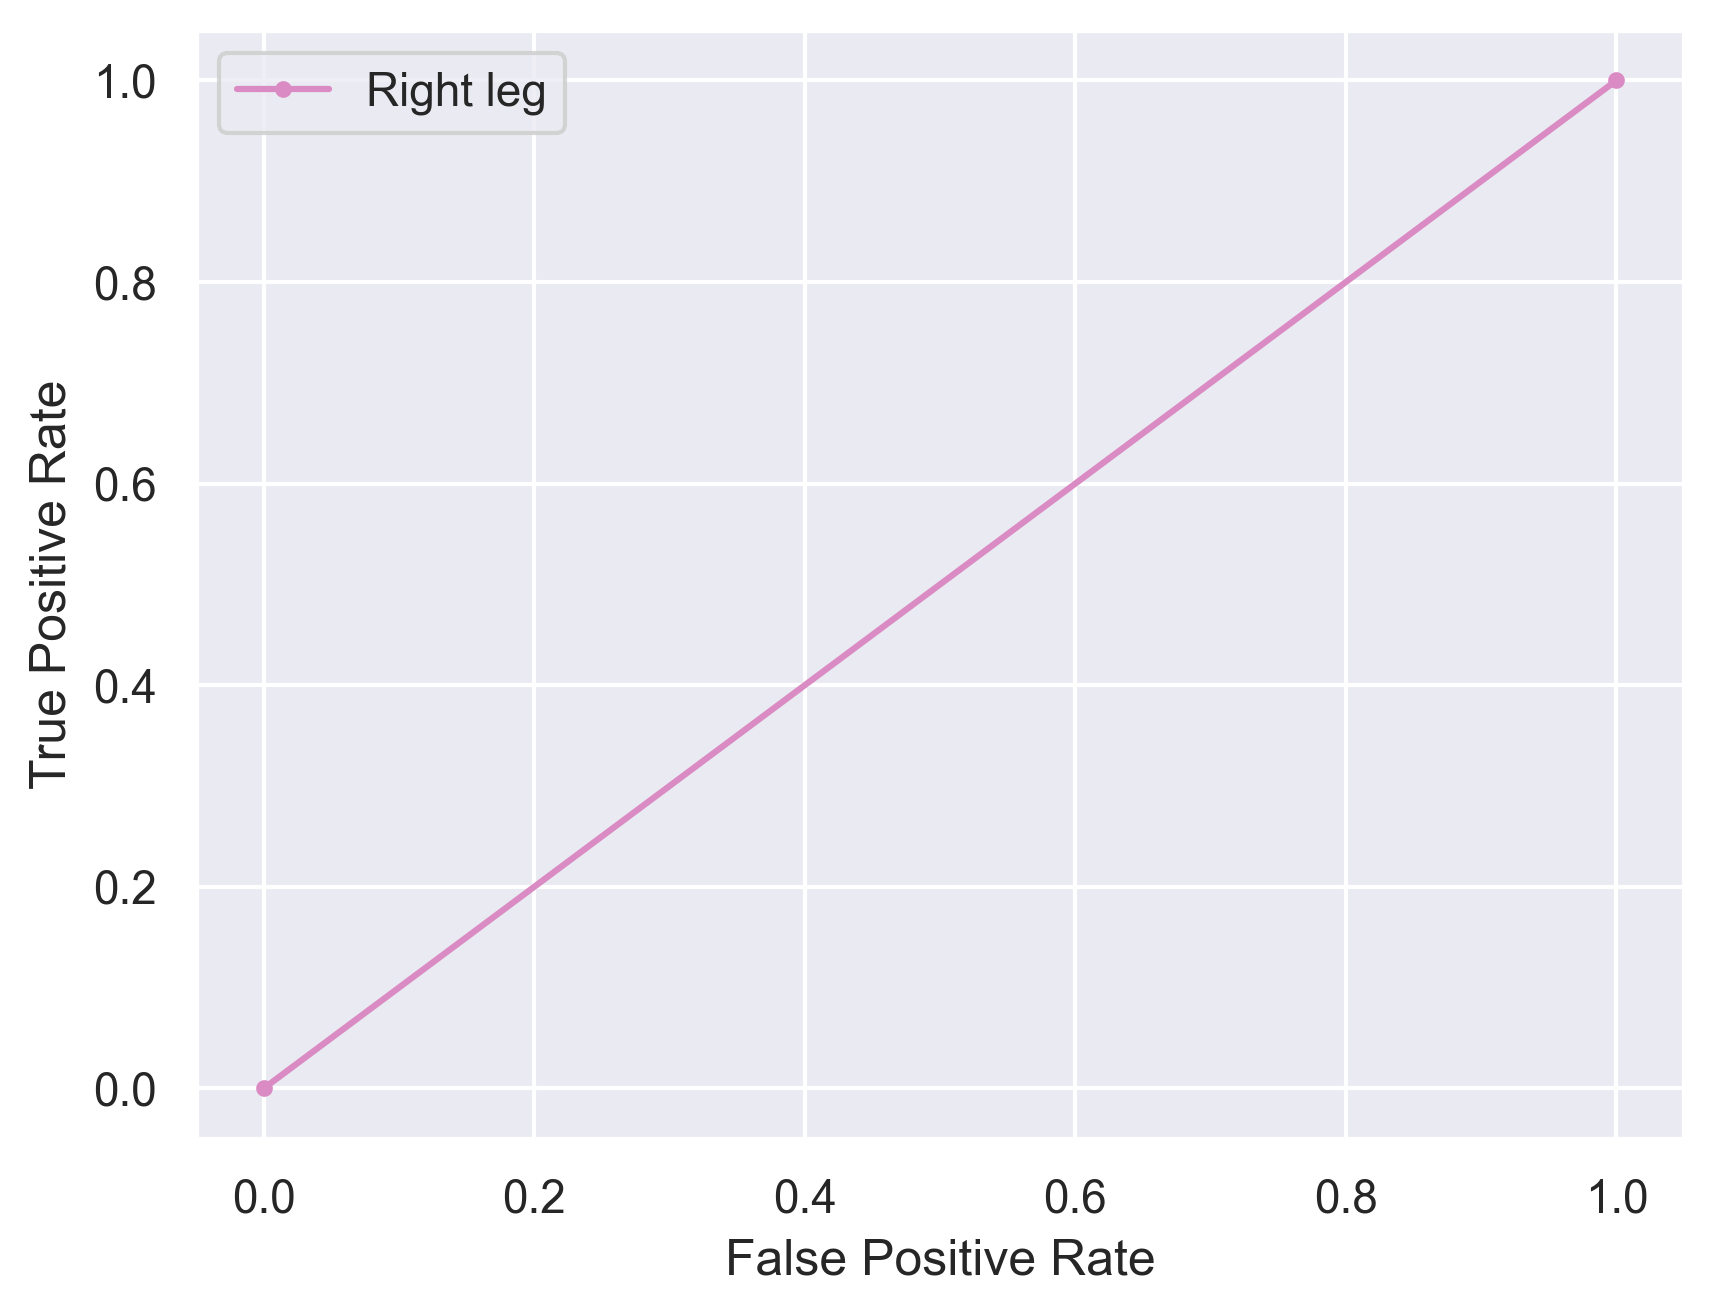
\includegraphics[width=\textwidth]{figures/Results/v1/roc/bp.png}
      \caption[]{Body Part Problem Set}
      \label{fig:bp_roc_v1}
  \end{subfigure}
  \hfill
  \begin{subfigure}[b]{0.4\linewidth}
      \centering
      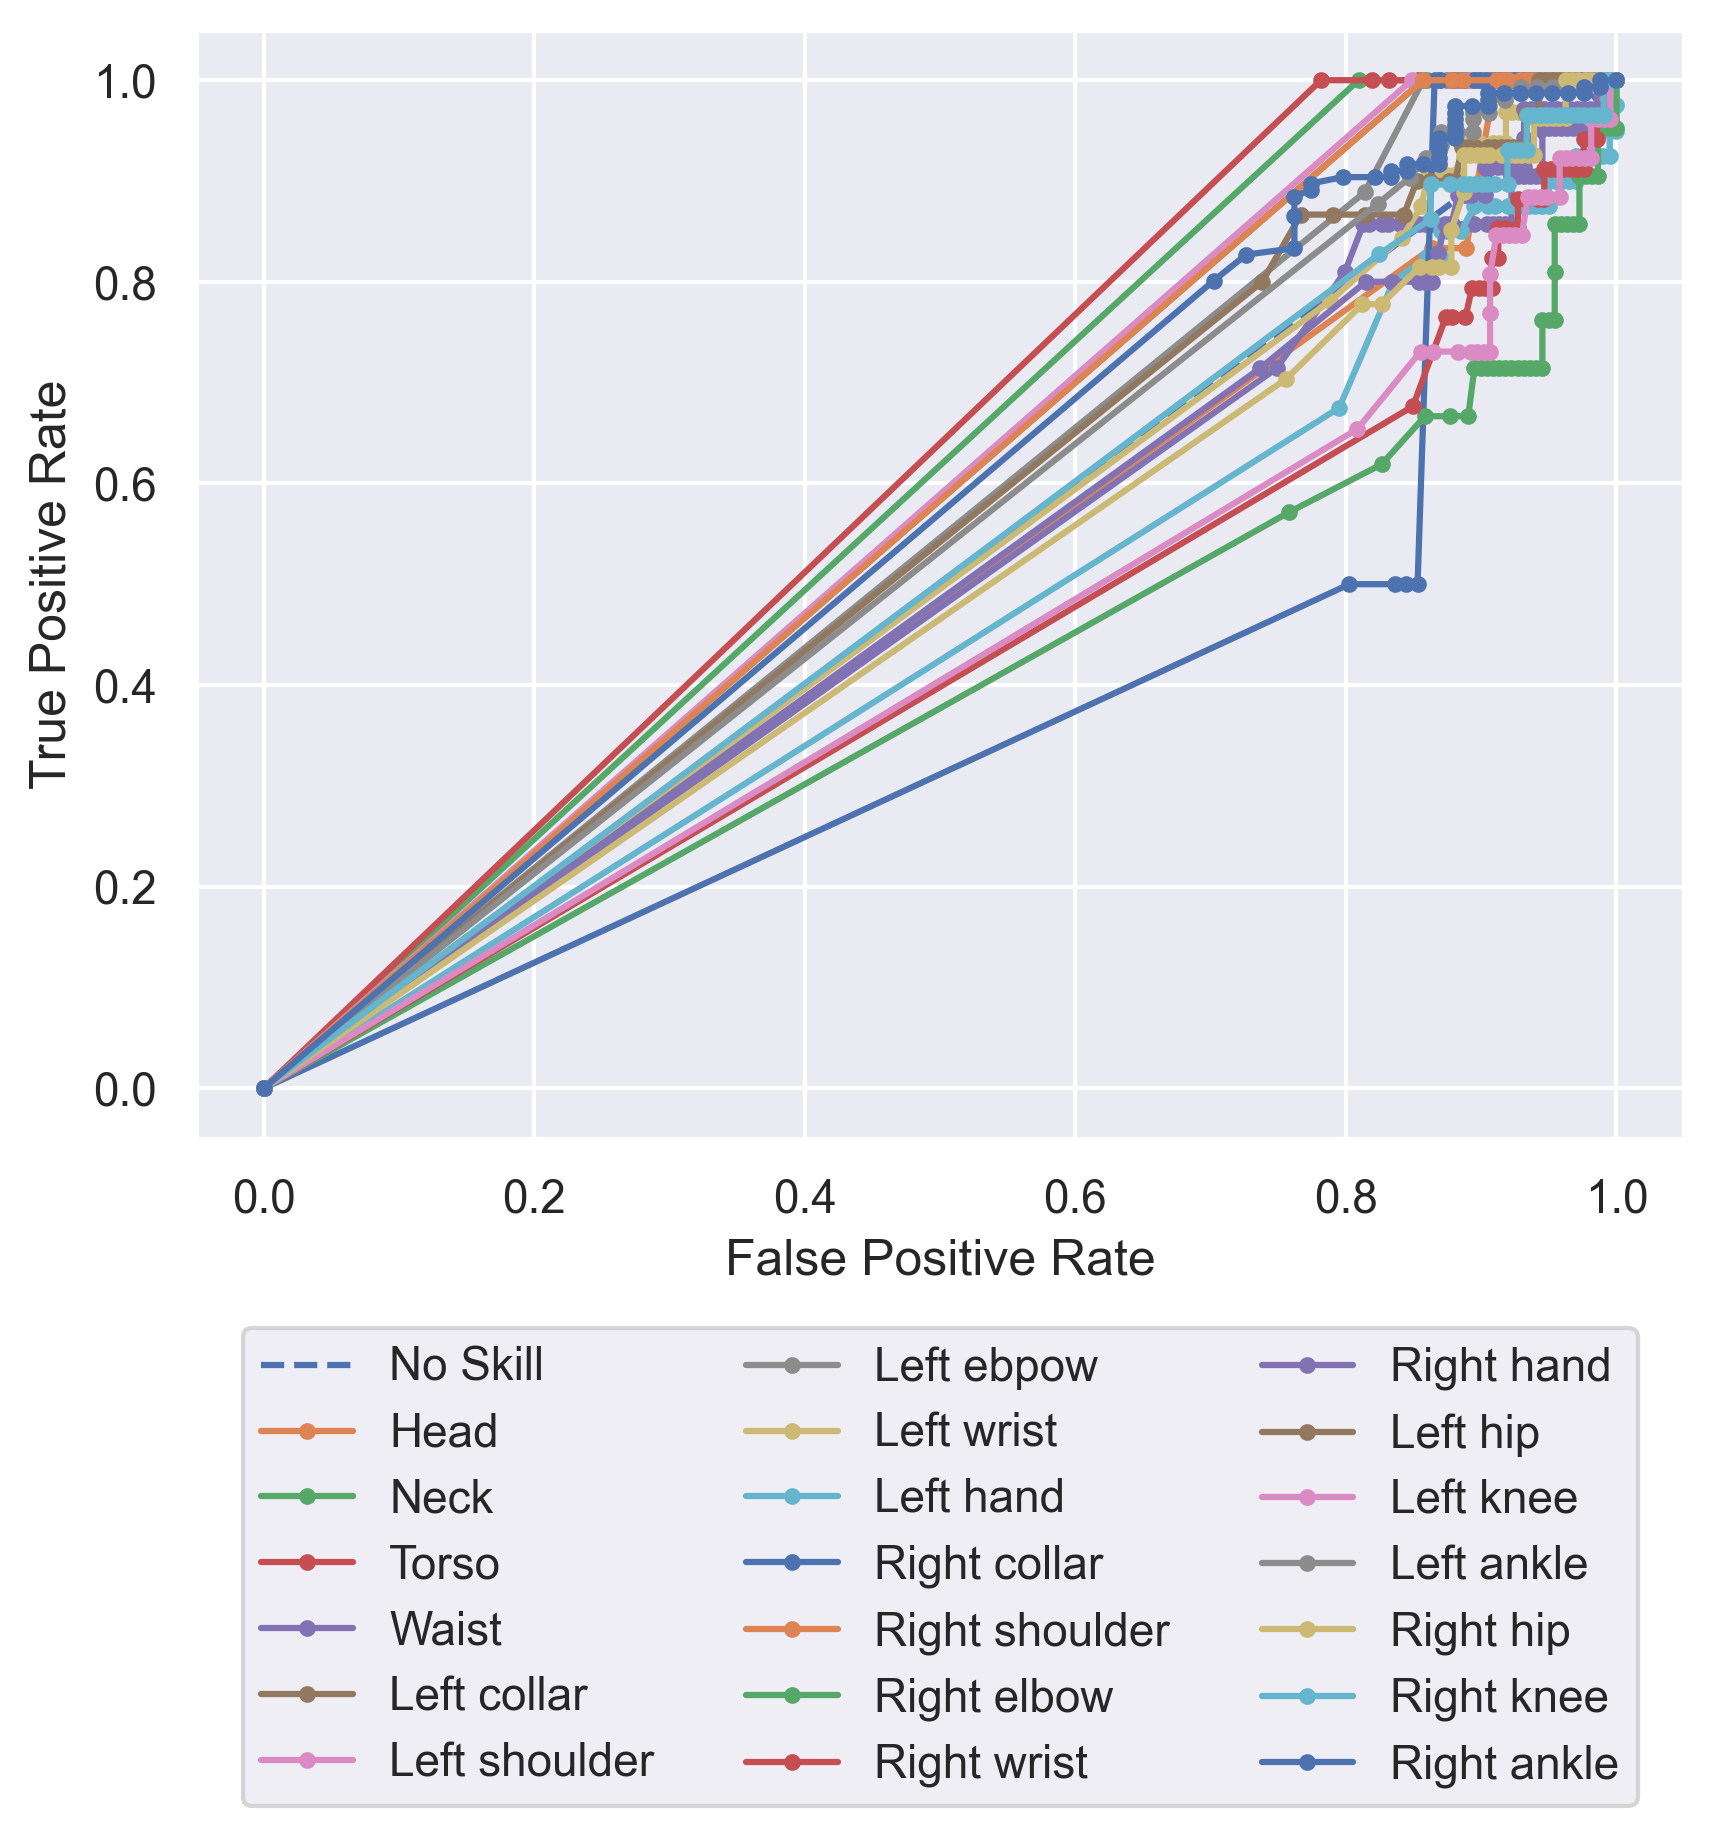
\includegraphics[width=\textwidth]{figures/Results/v1/roc/jt.png}
      \caption[]{Joint Problem Set}
      \label{fig:jt_roc_v1}
  \end{subfigure}
  \caption[ROC Curves of FESDModelv1]{The ROC curves of FESDModelv1.}
  \label{fig:roc_v1}
\end{figure}

The model is most accurate when predicting the body part problem set according to the calculated F1 score. However, there is a discrepancy between the F1 score, which is around 0.87, and Cohen's Kappa metric, which is only around 0.22. The reason for this discrepancy can be seen when considering the confusion matrix for each of the body parts. This can be seen in figure \ref{fig:conf_v1_bps}. While the model predicts that there is no error quite well, it does not predict errors well.

\begin{figure}[!htbp]
  \centering
  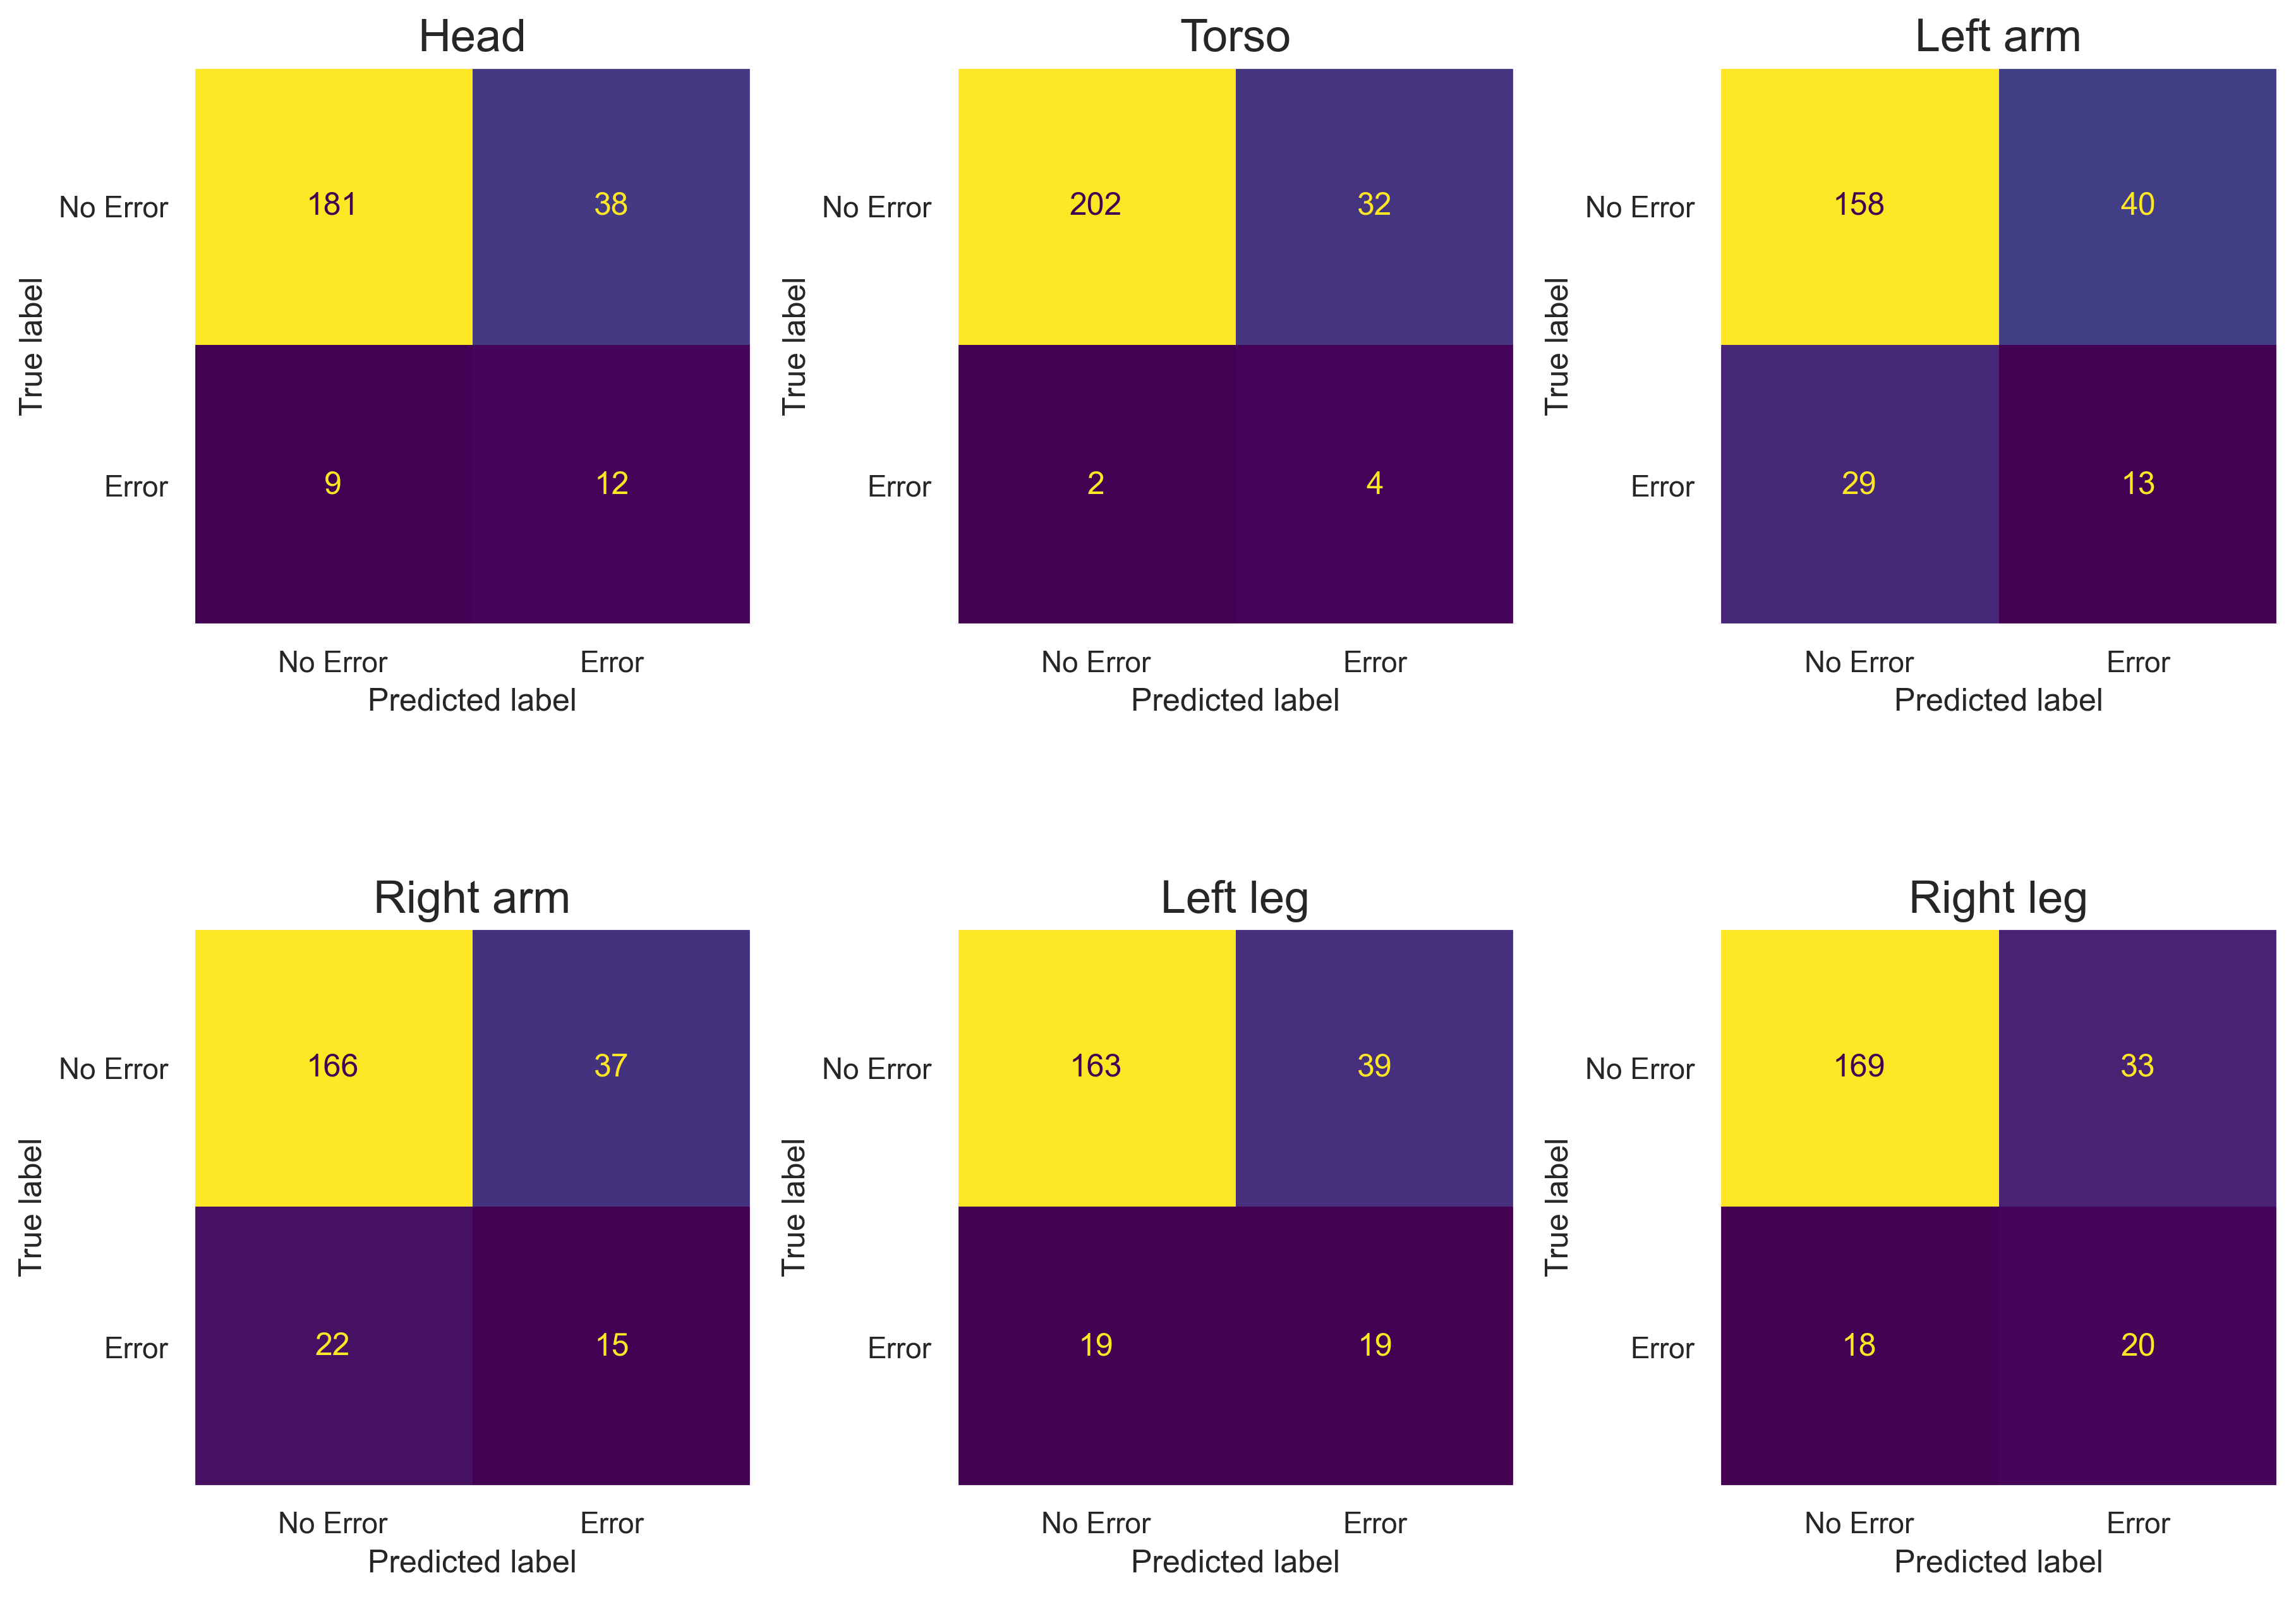
\includegraphics[width=.8\linewidth]{figures/Results/v1/confusion/body_parts_part.png}
  \caption[Confusion matrix of FESDModelv1 for each Body Part]{The confusion matrix of each body part for FESDModelv1 for the body part problem set.}
  \label{fig:conf_v1_bps}
\end{figure}

When only considering the accuracy of FESDModelv1 when predicting the joint problem set, it seems that FESDModelv1 is predicting the error labels well. However, since the results are taken as the average the individual results have to be investigated to get a clear picture of the results. Figure \ref{fig:conf_v1_jts} shows the confusion matrix of each joint on the test dataset. It can be seen that each joint is only predicting either no error or error depending on the joint. This is probably due to the unbalanced nature of the dataset.

\begin{figure}[!htbp]
  \centering
  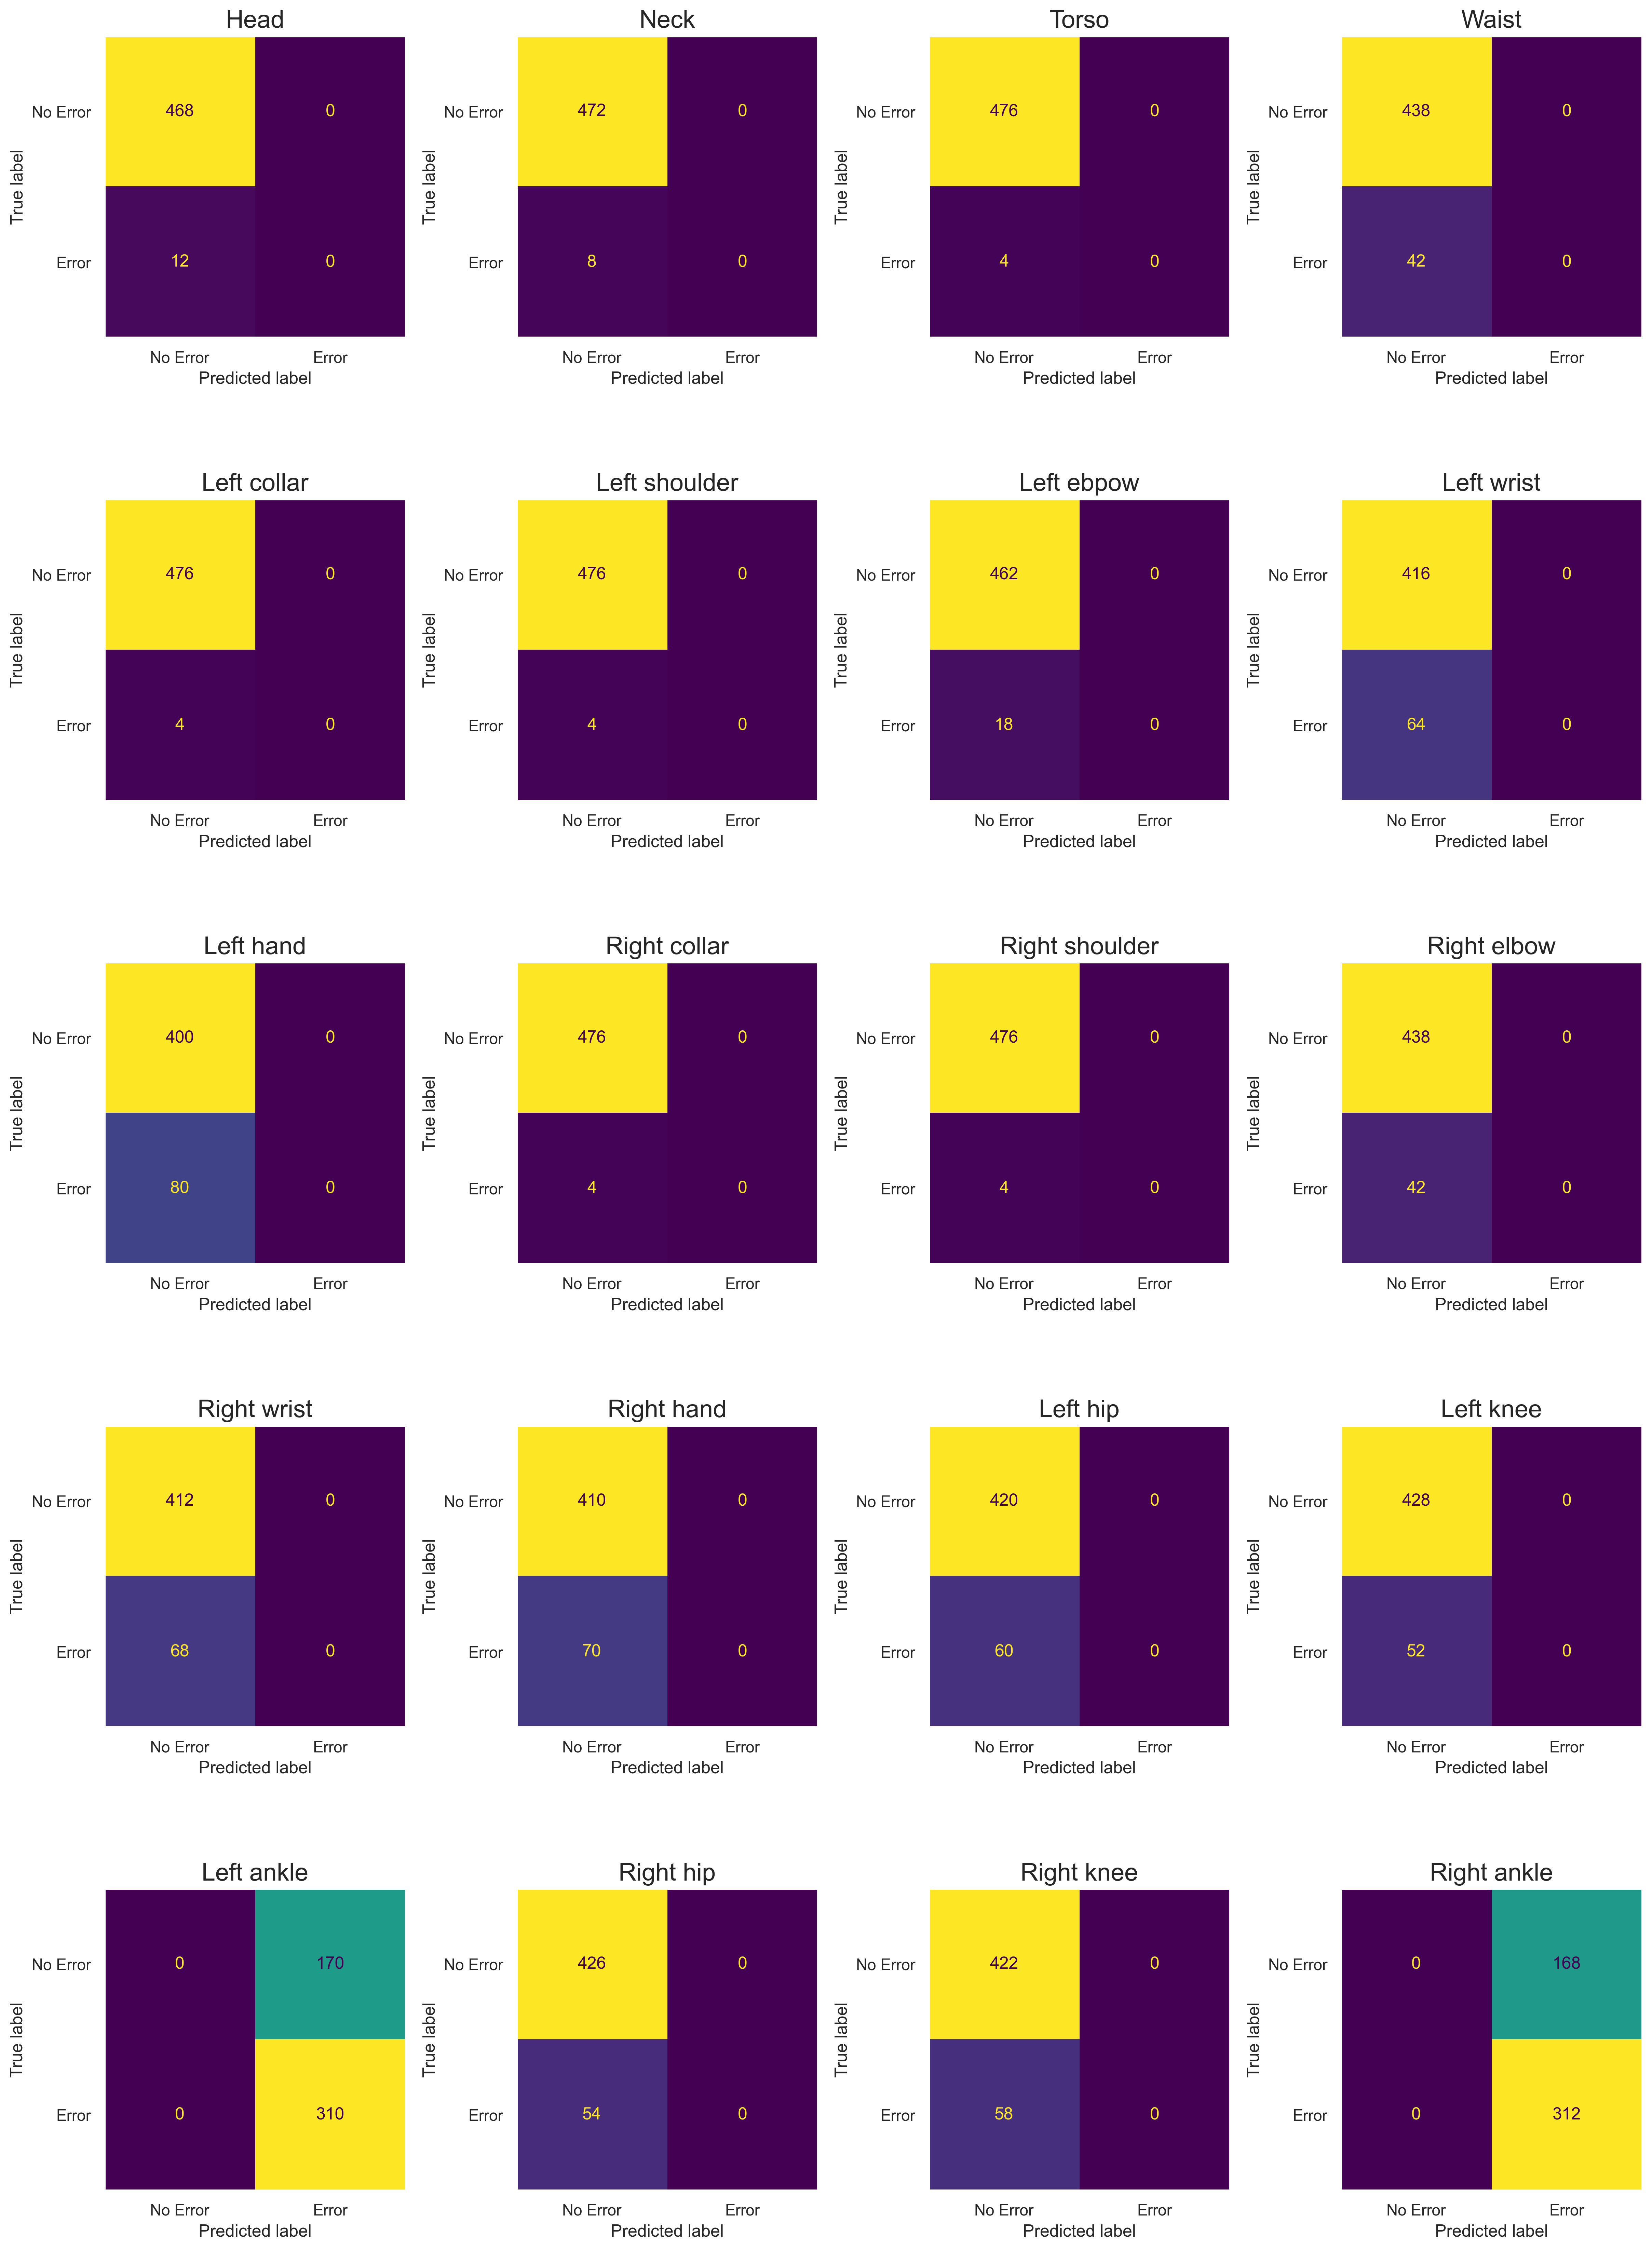
\includegraphics[width=.8\linewidth]{figures/Results/v1/confusion/joints_joint.png}
  \caption[Confusion matrix of FESDModelv1 for each Joint]{The confusion matrix of each joint for FESDModelv1 for the joint problem set.}
  \label{fig:conf_v1_jts}
\end{figure}

The best results are achieved using the half-body problem set. In Figure \ref{fig:conf_v1_hbs} the confusion matrix for the upper and lower body can be seen. The matrices indicate that FESDModelv1 is more accurate when detecting errors for the lower body than for the upper body. This is also reflected by the ROC-Curve seen in figure \ref{fig:hb_roc_v1}, which shows that the lower body is achieving better results than the upper body.

\begin{figure}[!htbp]
  \centering
  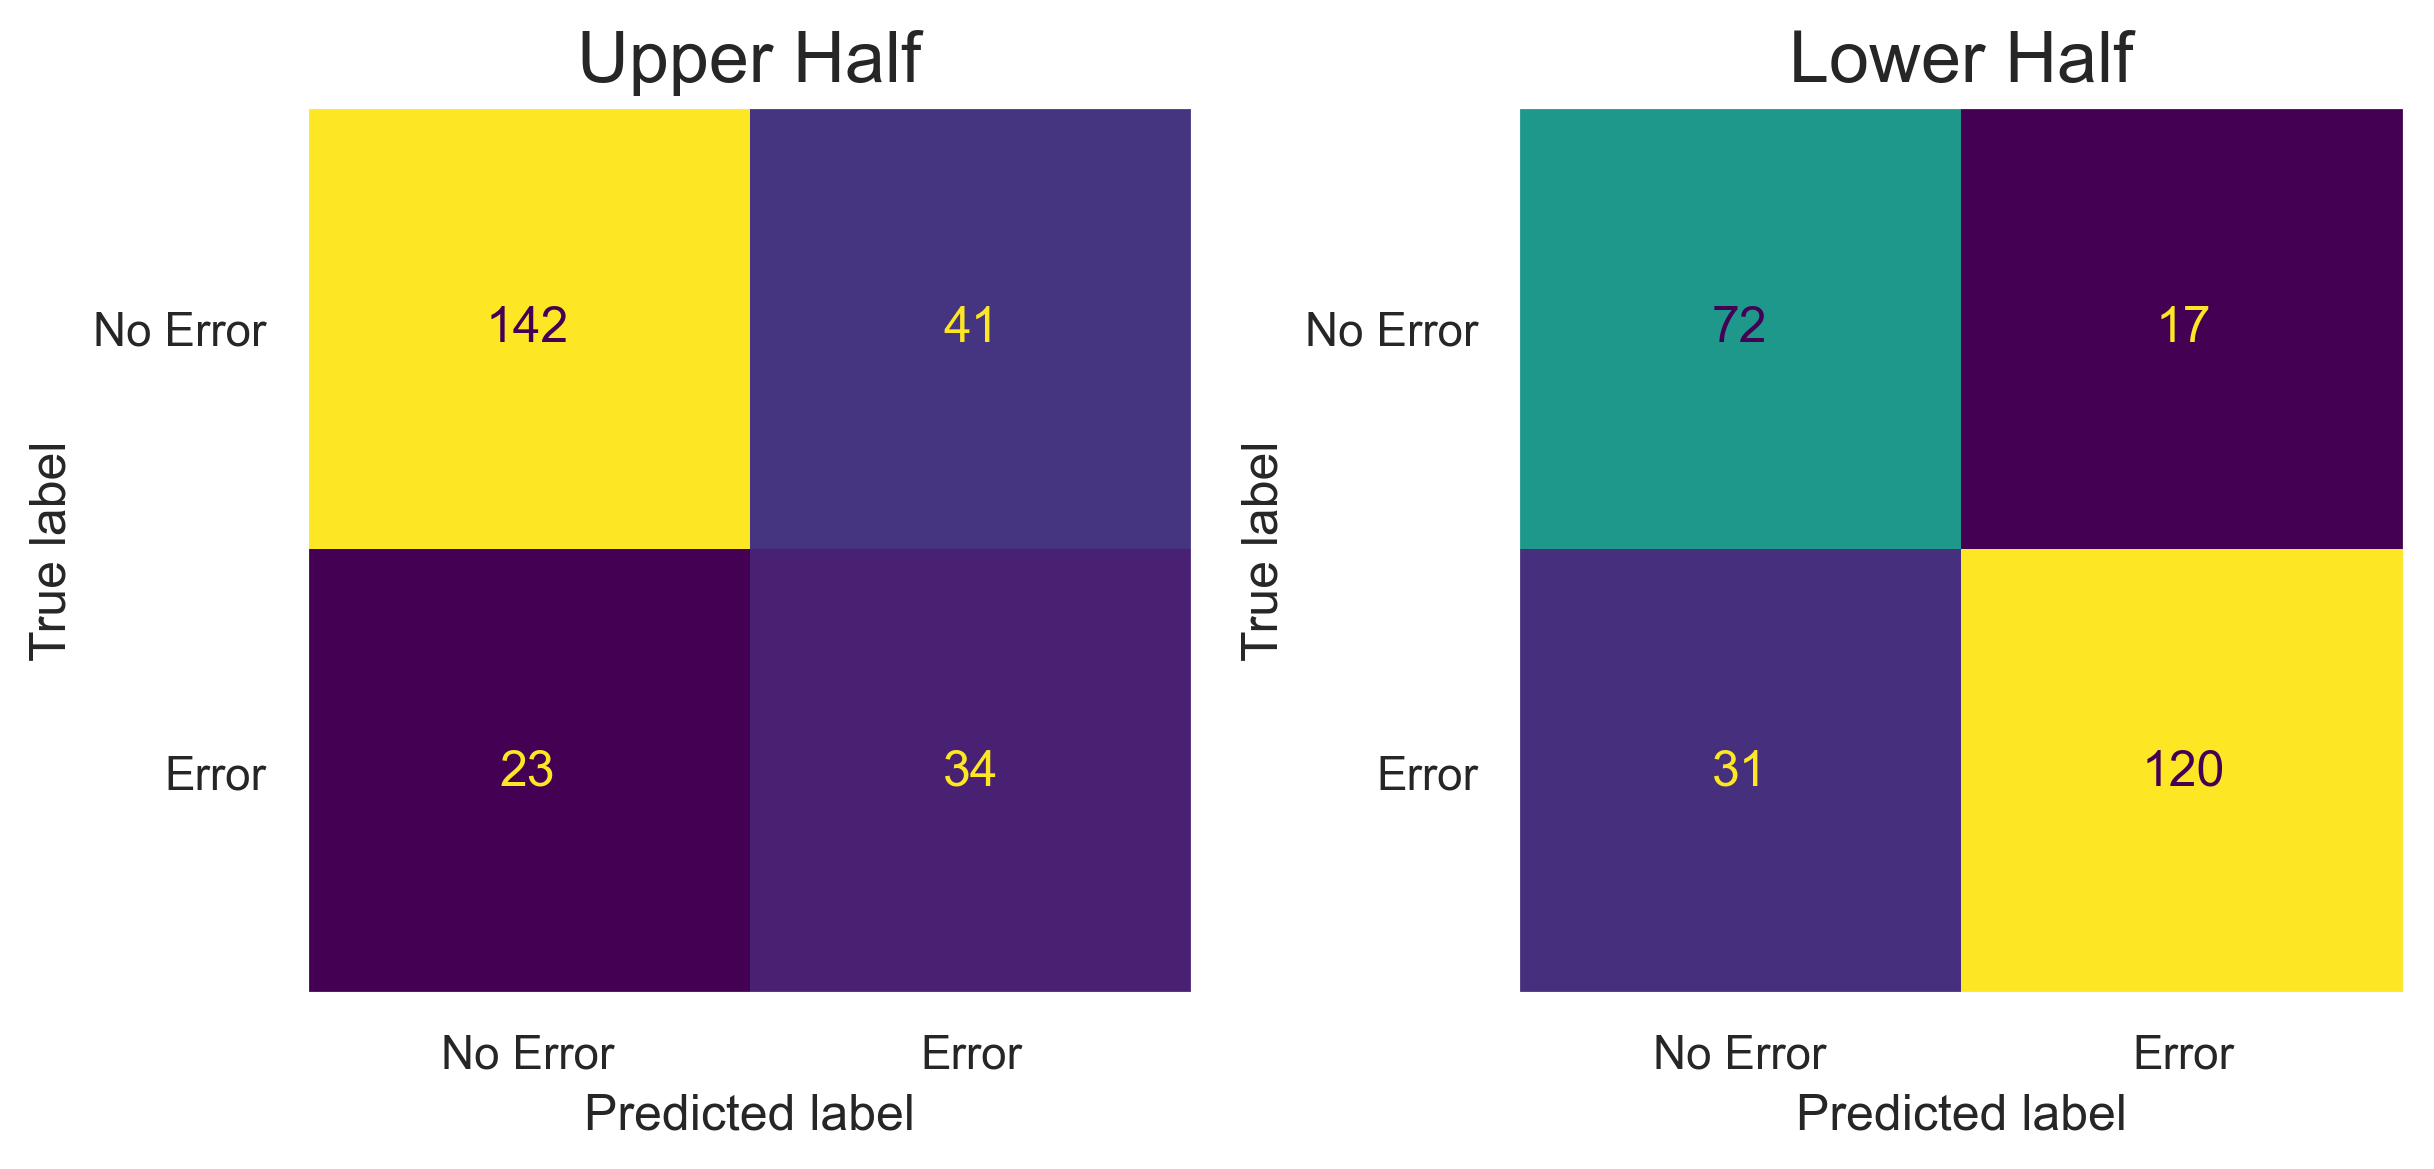
\includegraphics[width=.8\linewidth]{figures/Results/v1/confusion/body_halves_half.png}
  \caption[Confusion matrix of FESDModelv1 for each Body Half]{The confusion matrix of the upper and lower body for FESDModelv1 for the body half problem set.}
  \label{fig:conf_v1_hbs}
\end{figure}

\FloatBarrier